\section{Rappels}

\frame
{
	\frametitle{Notions abord�es au cours pr�c�dent}
	
	\begin{itemize}
		\item SOP = Service Object Pair.
		
		\begin{center}
			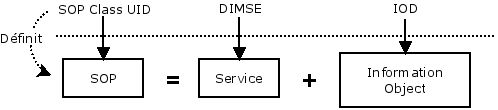
\includegraphics[width=.8\linewidth]{./figures/sop-definition.png}
		\end{center}
		
		Pour clarifier un peu : Object $\rightarrow$ \emph{Information Object} (\emph{IO}).
		
		\item Standard = annuaire.
		SOP Class UID vous permet de trouver � quel service et quel IOD il correspond.
		
		\item Attribut : une valeur.
		
		\item Module : ensemble d'attributs li�s.
		
		\item IOD = Information Object Definition.
		
		D�finit les modules (et donc les attributs) qui doivent �tre pr�sents pour un IO sp�cifique.
		
	\end{itemize}
}

\frame
{
	\frametitle{Information Object Defintion (IOD)}
	
	\begin{center}
	Ins�rer sch�ma de d�finition de l'IOD
%		\includegraphics[width=.8\linewidth]{./figures/iod-definition.png}
	\end{center}
}
